\documentclass[../main.tex]{subfiles}

\begin{document}

\subsection{Experimental Design}
\subsubsection{Participants}
%TODO: who were the participants, how many, what were the controls

\subsubsection{Imaging}
%TODO: Describe the imaging procedure for MEG and MRI

\subsubsection{Stimulus and Design}
%TODO: Show example stimulus, describe the experiment

\subsection{MEG Analysis}
\subsubsection{Preprocessing}
MEG analysis was performed in Python with the MNE-Python package \citep{mne}. Analysis was performed on 204 planar gradiometers (the 102 magnetometers were not used for analysis). Epochs were rejected for a subject if maximum peaks for any gradiometer exceeded a threshold of $4000\times10^{-13}  \frac{T}{m}$. MEG data was then band-pass filtered from 2-40hz, removing any potential low-frequency artifacts and unused high-frequency data. Independent component analysis (ICA) for each subject was calculated to remove artifacts caused by ECG and EOG artifacts. ICA performs source separation for statistically independent components of signals. Eighty independent components were generated for each subject, and independent components resembling ECG and EOG artifacts were visually selected and then excluded from the filtered MEG dataset. An example of these components is seen in figure \ref{ica_exclude}. Here, we see that the left component represents artifacts resulting from eye blinks (EOG), while the right component represents ECG artifacts. Trials were epoched from the onset of a gabor patch stimulus to 400 milliseconds after stimulus onset, with 16 time points for each epoch. Five hundred epochs were used for each subject.

\begin{figure}[h]
    \centering
    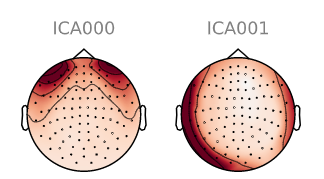
\includegraphics{figures/methods/ica_figure.PNG}
    \caption{Example ICA Components to be Excluded. Left: EOG artifact, Right: ECG artifact}
    \label{ica_exclude}
\end{figure}

\begin{figure}[h]
    \centering
    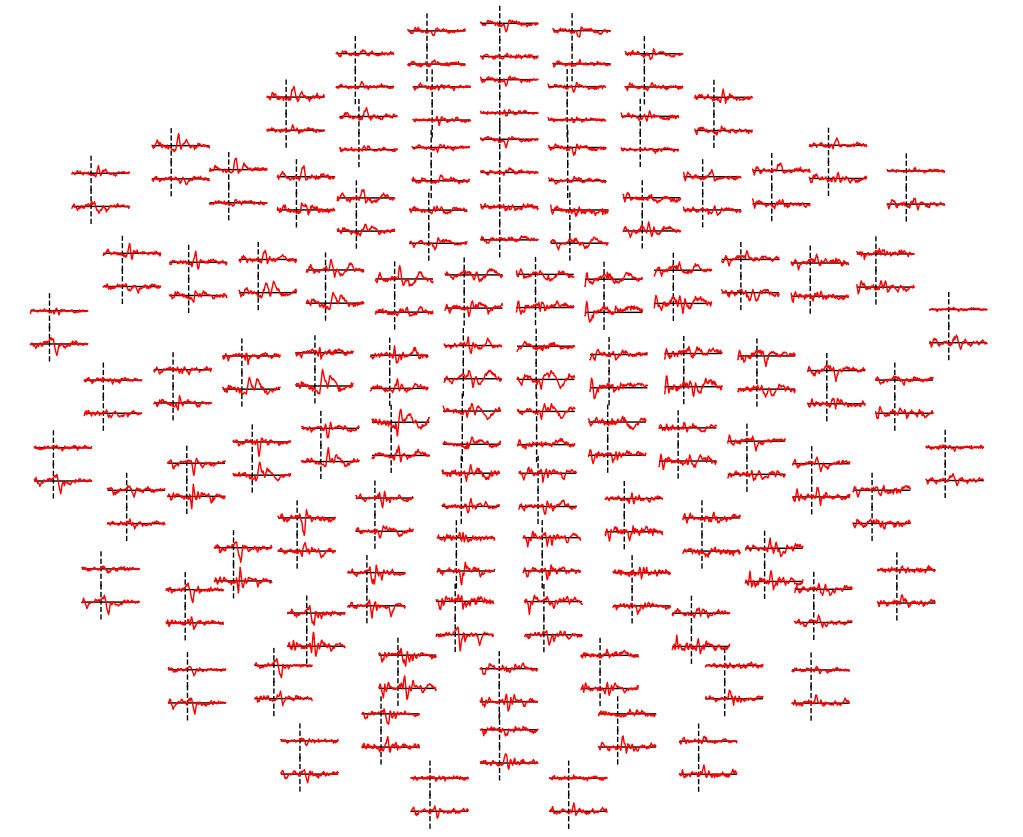
\includegraphics[scale=0.8]{figures/methods/good_topomap.PNG}
    \caption{Example of a Good ERF for a Subject}
    \label{good_topomap}
\end{figure}

\subsubsection{ERF Analysis}
The averaged evoked responses for each subject were measured to ensure that visual responses
appeared in the occipital area as expected. Time-locked epoch responses were averaged over all
trial blocks for each subject at each electrode and visually analyzed for aberrations. In a good subject, like in figure \ref{good_topomap}, we get evoked responses in left hemisphere occipital and temporal electrodes around 0.2 seconds after the stimulus is shown. The stimulus was only shown in the right visual field, so there is limited activation in the right hemisphere.

\subsection{Source Localization Analysis}
In source localization analysis, we estimate an inverse solution, i.e. the locations of underlying neural sources corresponding to MEG sensor readings \citep{mne}. The goal is to convert from sensor space, or the readings at MEG electrodes, to the source space, or readings on the cortical surface. To generate a source localization estimate of our MEG data, we followed the basic process outlined by MNE-Python \citep{mne}. This first required pre-processing the MRI data for each subject. We first computed the cortical surface reconstruction from each subject's MRI using FreeSurfer's recon all. We then used the skull stripping approach \citep{segonne_2004} implemented in FreeSurfer as mri watershed. Next, we performed co-registration with our MRI and MEG data, lining up the MEG sensors with the MRI reconstruction according to fiducial markers on the scalp. This aligns the coordinate systems of the MEG space and MRI space. Finally, we performed the mri watershed procedure again in the new coordinate system.

We next compute a solution to the forward problem for each subject. The forward problem involves computing the external magnetic field at various sensor locations on the scalp resulting from primary currents \citep{mosher99}. MEG electrodes read both primary and secondary currents; primary currents represent microscopic cellular currents that are associated with cognitive processes, while secondary currents are associated with macroscopic electric fields that we are less interested in \citep{mosher99}. To solve the forward problem, we first compute the source space locations for each subject, i.e. the locations of elementary dipole sources that we compute the forward operator at \cite{mne}. Each dipole is analogous to a sensor location located on the cortical source. To compute these locations, we inflate our computed cortical surface into a sphere, and overlay an octahedron onto it. We then subdivide this octahedron 6 times (oct6), giving us 4098 dipole locations for each hemisphere \cite{mne}. We then calculate the BEM solution with MNE-python, using the linear collocation algorithm \citep{mosher99, hamalainen89} for each subject. Using the BEM solution, source space, and the evoked response for a subject, we compute the forward solution as implemented in MNE-python.

Once the forward solution is calculated, we are able to estimate the inverse solution with MNE \cite{mne}. We first use a weighted minimum norm estimate \citep{fuchs_1999, lin_2006} with a loose orientation approach \citep{lin_2005} to estimate source current densities. This approach uses our forward solution and the covariance matrix from our epoched data. Source estimates are then computed from the source current densities using dynamic statistical parameter mapping (dSPM) \citep{DALE200055}. These source estimates contain source amplitudes epoched at stimulus onset for each of the 4098 sources in each hemisphere at 16 timesteps, and can now be incorporated into a decoding pipeline as numpy arrays. An example source estimate can be seen in \ref{source_ka}. To validate the results of our source localization estimates of the inverse solution, we plotted the average source space response after stimulus onset for each subject, and compared each source space response to the corresponding sensor space response. We checked that source space responses occurred in the occipital lobe, and ensured that source space peaks occurred at the same time as sensor space peaks.

\begin{figure}[h]
    \centering
    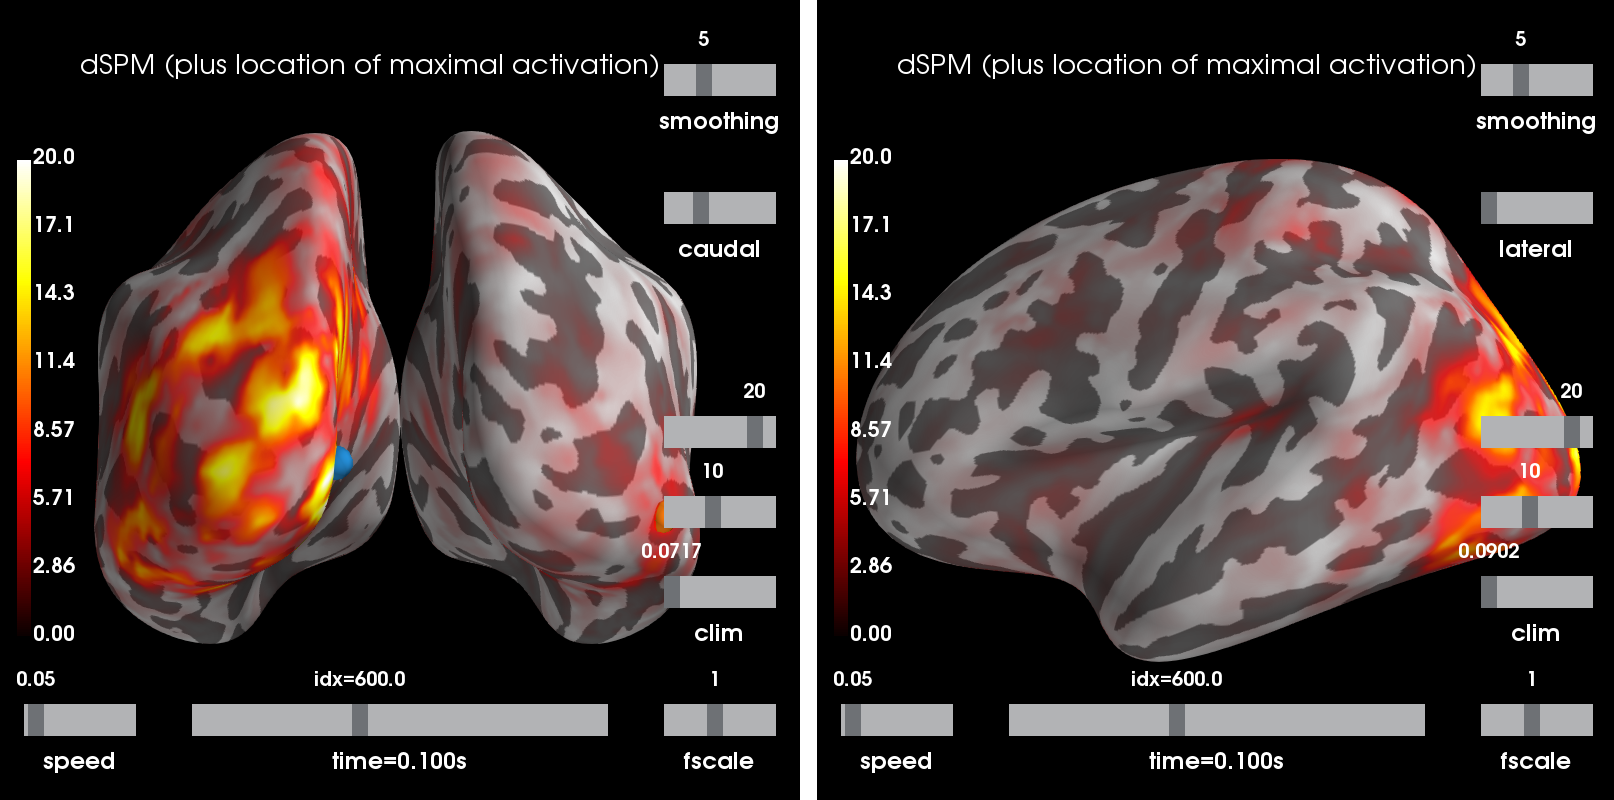
\includegraphics[scale=0.4]{figures/methods/source_loc_KA.png}
    \caption{Average source estimate for subject one subject at 100 ms after stimulus onset. Activations originate in the occipital lobe.}
    \label{source_ka}
\end{figure}

\subsection{Statistical Analysis Methods}
\subsubsection{Data Processing}
Analysis was performed in Python using the Keras \citep{chollet2015keras} library from TensorFlow \citep{tensorflow2015-whitepaper}, decoding libraries from MNE-Python \citep{mne}, and the scikit-learn library \citep{scikit-learn}. Data was split into training sets of 500 trials for each subject with 100 trials of test trials. Trials were time-binned from 0-0.4 seconds at 0.025 second intervals to account for the 40hz MEG data. In the experimental design, Gabor patches were shown at random orientations from 0-180 degrees. For decoding analysis, these Gabor patches were binned into $n$ different classes for decoding model classification. Bins were used because it was difficult to perform a circular regression of orientation angles, especially with relatively few data points. Bin sizes were chosen as a balance between minimizing the angular width of each bin (modeling the original 180 possible Gabor orientations more closely) and maximizing the number of features per bin (giving more trials for each class to improve model performance). Each bin was normalized to have the same number of features by filtering out data points for bins that had more data points than the smallest bin. Decoding models were tested with 4, 8, and 9 bins, and final analysis was performed with 8 bins. Individual models were trained for each subject before calculating group averages to account for individual differences in MEG response.

Gabor patches were binned in bow-tie ranges as shown in \ref{gabor_bins}. Because a Gabor patch oriented at $n$ degrees is functionally identical to a Gabor patch oriented at $n + 180$ degrees, these bow-tie ranges for classification ensure that we do not put two functionally identical Gabor patches into two separate bins. We center these bow-ties around the horizontal and vertical axis, as well as the two diagonals. For 4 classes, class 0 corresponds to Gabor patches oriented from (337.5-22.5) degrees and (157.5-202.5) degrees, class 1 from (22.5-67.5) and (202.5-247.5) degrees, class 2 from (67.5-112.5) and (247.5-292.5) degrees, class 3 from (112.5-157.5) and (292.5-337.5) degrees. If a Gabor patch were to have an orientation of 125 degrees, it would be binned into class 3, and the label of "3" would be used as the classification label in machine learning decoding models. 

\begin{figure}
    \centering
    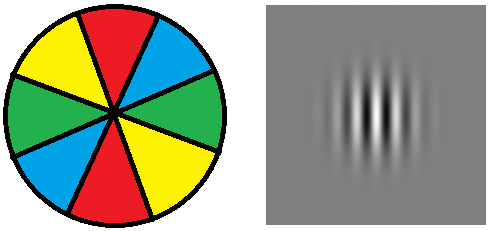
\includegraphics{figures/methods/gabor_bins.png}
    \caption{Right: Bins for four classes. Sectors of the circle with the same color correspond to the same bin. Left: Example Gabor patch oriented at 0 degrees. This Gabor patch would be binned into the red bin, as it could be regarded as having an orientation of 0 degrees (the top red sector) or 180 degrees (the bottom red sector).}
    \label{gabor_bins}
\end{figure}

Decoding model accuracy was calculated with k-fold cross-validation, where the accuracy metric was the number of correct labels predicted by the model out of the total number of labels predicted. Model accuracy was then compared with the results of a permutation test, in which we shuffled around the training and test labels of the data set to create a null distribution with which to test our null hypothesis. Models were run using both senor space (MEG electrodes) and source space (source estimates) data. There were many more MRI vertices than MEG electrodes, so the weight matrices for the source localization models were much larger than the electrode models. Thus, hyperparameters were tuned differently for the MEG electrode models and source localization models.

The final data had the shape $\mathrm{X} = $ ($n$ epochs $\times$ $m$ sensors/sources $\times$ $t$ time steps) and $\mathrm{y} = $ ($n$ epochs), $1 \leq \mathrm{y}_i \leq 8$, $\mathrm{y}_i \in N$

\subsubsection{Permutation Test}
A permutation test was used to determine the statistical significance of the various decoding experiments. Here, features will refer to the $n \times m \times t$ MEG data matrix with $n$ epochs, $m$ electrodes, and $t$ time steps, and the $n$ labels refer to the classification bins of the stimulus Gabor patches, where label $i$ is the label corresponding to the feature data for epoch $i$. In this test, each model was trained 10 times on a shuffled data set (features and labels shuffled together) to determine the performance of the experimental model.  The experiment was run another 100 times with shuffled labels, i.e. the permutation test. In each of these 100 iterations, the data was shuffled as before, with features and labels together, but labels were then shuffled again, separate from the corresponding feature vector. This label shuffling removes any structured relationship between features and labels. Thus, these permuted trials will give us a null distribution for our experiment, where the null hypothesis suggests that there is no structured relationship between the MEG features and the labels. To calculate a p-value, the performance of each of the $n = 100$ permutation trials is compared against the $m = 10$ experimental trials, as follows. 
$$\rho = \frac{1}{m}\sum_{i=1}^{m}{\frac{1}{n}\sum_{j=1}^{n}{f(exp_i, perm_j)}}$$
$$f(exp_i, perm_j) = 1 \mbox{ if } perm_j \geq exp_i \mbox{, } 0 \mbox{ otherwise}$$
$$ exp_i = \mbox{ performance of experimental trial } i$$
$$ perm_j = \mbox{performance of permutation trial } j $$

This can be thought of as the proportion of permutation trials that outperform a particular experimental trial, averaged over all of the experimental trials. A low p-value suggests that the experimental trials are on the tail end of the null distribution, suggesting that there may be a structured relationship between the features and labels of the dataset, disputing the null hypothesis.


\subsubsection{Sliding Logistic Regression Model}
The first machine learning model used for our control model was a sliding logistic regression model, which calculates a separate accuracy for each time step of our MEG input signal. For 16 time steps, we calculate 16 different logistic regression weights, and update these weights using a gradient descent procedure while training. The model was regularized with an elastic net regularization term, which acts as a combination of L1 and L2 regression. This regularization term helps enforce sparsity within our model and prevents weights that are too large, combining the traditional benefits of L1 and L2 regularization. The model also used a "select K best" routine that selects the $K$ best features from the model, based on their contributions to the accuracy. We then had to tune the hyperparameters for these additions to our model, namely the size of $K$, the ratio between L1 and L2 loss for elasticnet, and the regularization parameter $C$. The hyperparameters were tuned to get the best cross-validation accuracy for 500 trials.

Here, logistic regression models $\mathrm{Pr}(\textrm{orientation of stimulus } (\mathrm{y}_i) = \omega | \mathrm{X}_i)$. We use multinomial logistic regression for multi-class prediction with logistic regression. The logistic regression model was used for its simplicity and interpretability. The model is relatively easy to implement, especially with the machine learning packages that are already built into scikit-learn \citep{scikit-learn} and mne-python \citep{mne}. The model has only one layer, making it relatively fast to run the model and tune the model parameters. This also means that we can interpret the weights quite easily, as there is a one-to-one correspondence between a particular weight and feature from an MEG electrode or MRI vertex. This tells us that if a particular weight has a high value, the corresponding electrode/vertex is weighted highly in the model. Further, the logistic regression model outputs a probability for each class, which is useful in serial dependence analysis.

\subsubsection{Support Vector Machine Model}
%TODO: SVM info

\subsubsection{Neural Network Models}
We also ran experiments with two neural network based models: a sliding neural network (SNN) and a wavelet-based convolutional neural network (CNN). Each of these models was built using the Keras framework from TensorFlow \citep{chollet2015keras, tensorflow2015-whitepaper}. The SNN and CNN were used because they had the potential of modeling higher-level features, like orientation, in the data. However, neural networks are generally less interpretable than regression models, and are much easier to overfit to a small data set. 

Similar to the sliding logistic regression model, the SNN calculates separate predictions and model weights for each time step in the input, but we instead train a neural network instead of a logistic regression model. The SNN is much more complex than the logistic regression model, as it has multiple layers, activation functions between each layer, and multiple hyperparameters to tune. Particularly, we have to choose the layer sizes and batch sizes. For each neural network, there were 3 dense network layers with relu activation functions and l1 and l2 regularization. The final output layer had a softmax activation function with $n$ outputs, where $n$ is the number of bins being classified. Accuracy metrics were generated using 5-fold Cross-Validation with 8 classes.

The wavelet CNN took a different approach to analyzing the data, generating a single classification for each epoch by looking at the wavelet transform of the epoch as a whole. For each epoch, a wavelet transform was generated for each electrode, with 5 frequency bands ranging from 5 to 40 hz over 16 timesteps, giving an input tensor of (204, 5, 16). This input tensor was then input to a convolutional neural network with 2 convolutional layers with relu activation functions and one dense output layer with a softmax activation function. We again use l1 and l2 regularization on each hidden layer of the neural network. If there were any relationship between responses at different frequency bands and stimulus orientation, this model would have a good chance of decoding this relationship.


\subsubsection{Inverted Encoding Model}
A final decoding approach was the use of the Inverted Encoding Model (IEM) \citep{Brouwer09, Brouwer, GARCIA2013515,sprague_serences_2013, sprague_saproo_serences_2015}. The IEM calculates the predicted responses of each classification channel based on the MEG data, rather than giving a class prediction. This model is well-suited for orientation decoding because it uses a cosine basis set to transform the input data, modeling the inputs better than a linear scale from 0 to 179. In the cosine basis set (shown in \ref{basis_set}, a perfect channel response centered at 160 degrees would propagate equally to the right and left and wrap around the unit circle, having a similar response at 140 degrees and 180 degrees, and 120 degrees and 20 degrees. This can be seen in \ref{ideal_chan_resp}. 

\begin{figure}
    \centering
    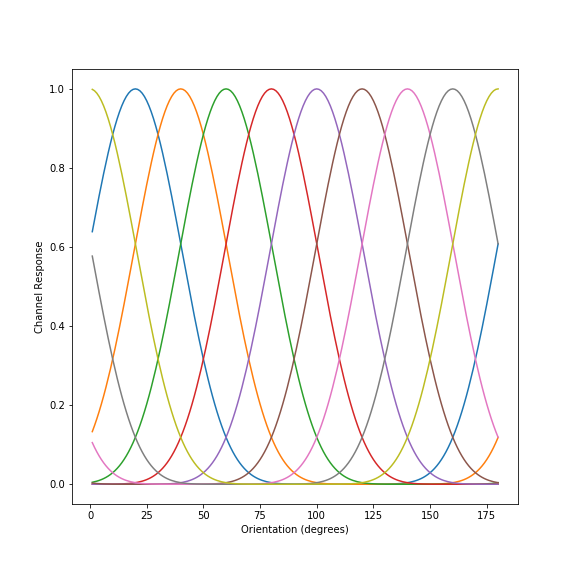
\includegraphics[scale=0.7]{figures/methods/basis_set.png}
    \caption{An example cosine basis set for 9 orientation classes. Each color represents the
    basis function for a single orientation channel, where the cosine function peaks at that
    orientation channel.}
    \label{basis_set}
\end{figure}

\begin{figure}
    \centering
    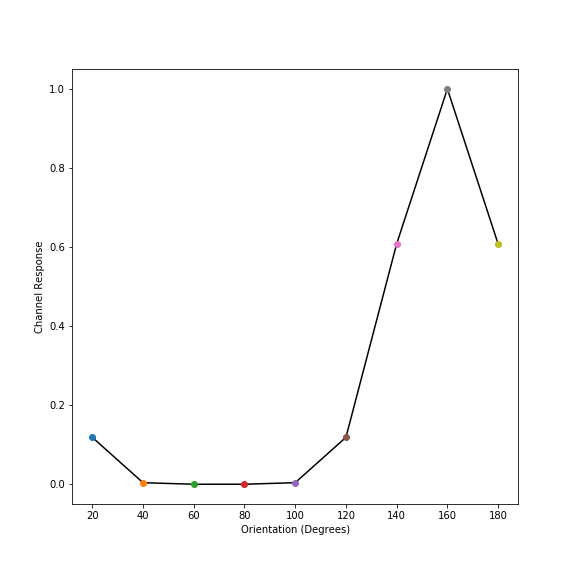
\includegraphics[scale=0.7]{figures/methods/ideal_chan_resp.png}
    \caption{The ideal channel response for a stimulus oriented at 160 degrees.}
    \label{ideal_chan_resp}
\end{figure}

To compute the predicted channel response for our MEG data, we first construct a hypothetical channel
response $\mathrm{C}$ with shape (number of epochs $\times$ number of orientation channels). This is computed by matrix multiplying a stimulus mask matrix by the cosine basis set. The stimulus mask has shape (number of trials $\times$ 180), where row $i$ has value 1 at the degree of trial $i$'s stimulus orientation, and 0 elsewhere. In the problem formulation of the IEM, there is the MEG input data, $\mathrm{B_{train}}$ with shape (number of epochs $\times$ number of MEG electrodes), which is related to the channel response set, $\mathrm{C_{train}}$, by the following formula:
$$ \mathrm{B_{train} = W C_{train}}$$
We first compute $\mathrm{\hat{W} = B_{train} C_{train}^T (C_{train} C_{train}^T)^{-1}}$, the linear least squares estimate for W in $ \mathrm{B_{train} = W C_{train}}$. We then solve for the predicted channel responses $\mathrm{C_{test}}$  of our test set, related to the test MEG data $\mathrm{B_{test}}$ by the formula $\mathrm{B_{test} = W C_{test}}$, which is estimated by least squares as 
$$\mathrm{C_{test} = (\hat{W}^T \hat{W})^{-1} \hat{W}^T B_{test}}$$

We then perform k-fold cross-validation to generate accuracy over all the trials, and perform this analysis at each timestep. The channel response is informative on its own, but we can also generate a classification for a trial by taking the argmax of the channel response (channel corresponding to maximum channel response) for a particular trial.

\subsection{Serial dependence Analysis}
A variety of methods were used to determine how the previous stimulus affected the perception of the current stimulus, i.e. serial dependence. 

\subsubsection{Behavioral Analysis}
Before performing decoding analysis for serial dependence, we performed the first serial dependence experiment outlined in \cite{fischer_whitney_2014} to determine if a serial dependence effect existed in our data. For each subject, we calculated the error for a trial (reported orientation - presented orientation), where positive values indicate errors in the clockwise direction. For each trial, we calculated the difference between the previous and current trial for each trial, where a positive value signifies that the previous orientation is more clockwise than the current orientation. We plotted the error on the y-axis and the previous-current trial difference on the x-axis. We then fit the error plot with a derivative of Gaussian (DoG) curve, allowing us to measure the amplitude of the serial dependence effect. This curve is modeled by the function, $y = (a b c) x e^{-(b x)^2}$, where $x$ is the relative orientation of the previous trial, $a$ is the amplitude of the DoG curve, $b$ is the DoG curve width, and
$c = \frac{\sqrt{2}}{e^{-0.5}}$.

Error bars were generated by bootstrapping the DoG curve fit 5000 times, sampling with replacement. To generate $P$ values for this DoG curve, a permutation test was again used, generating 100,000 DoG curves with shuffled data labels (relative previous orientation) for each iteration. The amplitudes of the permuted DoG fits were compared against the measured amplitude of the subjects, and the $P$ value was taken as the proportion of permuted amplitudes that were greater than or equal to the measured subject amplitude. This analysis was performed using the lmfit library for python \citep{newville_matthew_2014_11813}.

\subsubsection{Previous Orientation Decoding}
We then attempted to decode the orientation of the $(t-1)$th stimulus from the MEG response data corresponding to the $t$th trial. If the previous stimulus orientation biases the current stimulus orientation perception, then it's possible that a decoding model could reverse engineer this bias and decode the orientation of the previous stimulus. This analysis was computed with the same decoding model as the current stimulus decoding, but we shifted the data labels backward by one time step in relation to the data, such that the data at time $t$ was used to predict the label at time $t - 1$. We performed the same permutation test as in previous decoding models to test the significance of this previous trial decoding.

\subsubsection{Performance Bias Analysis}
We next investigated how the relative previous stimulus orientation affected the decoding of the current stimulus. We again calculated the relative previous stimulus orientation (previous orientation - current orientation) for each trial, where positive values indicate that the previous orientation was more clockwise than the current one. We then ran the same 5-fold cross-validation decoding process on our MEG data with the logistic regression model and the IEM model. For the logistic regression model, we generate prediction probabilities for each class for each trial, which represent the likelihood that the features for a trial represent a certain stimulus orientation. For the IEM, we generate the channel responses for each stimulus orientation bin for each trial. We can then bin these channel responses and class probabilities by relative previous orientation to reveal any relationship between model predictions and relative previous orientation. Each bin is normalized to have the same number of entries. We then center each channel response such that actual label of the data lines up with the same label for all trials. For example, if we align all responses to channel 5, and trial $i$ has a label of channel 3, we would roll the channel response for $i$ to places to the right. 

We then subtract the mean channel response from all bins, giving us the deviation of each bin from the mean. If there is any impact of serial dependence on decoding, we would expect to see channel response biased away from the mean in certain bins. To test how significantly each bin deviates from the mean, We perform another permutation test, this time shuffling the bin that each channel response falls into. We then calculate a $P$ value for each channel response in each bin as the proportion of permutations that have greater deviation from the mean than the measured channel response for said bin.

\end{document}